\sect{Overview}

\begin{figure}[ht!]
  \centering
  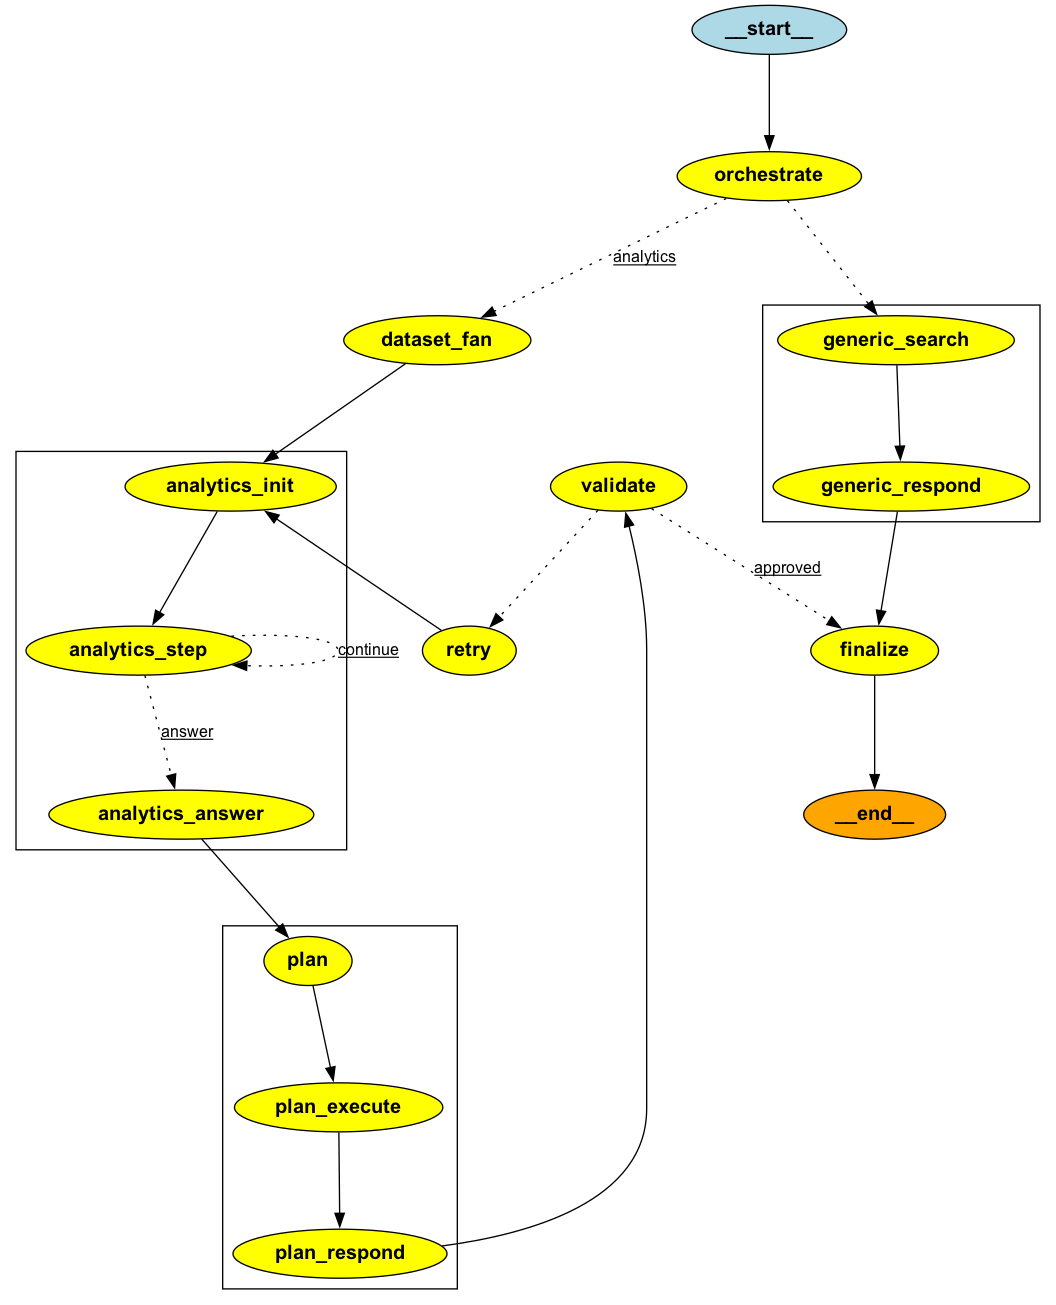
\includegraphics[width=0.4\textwidth]{graphics/graph-full.png}
  \caption{Full Agent Graph}
\end{figure}

The project implements a LangGraph-based analytics agent capable of answering
questions against CSV datasets, while also supporting a deterministic
plan-and-execute path and validation. The architecture combines:
\begin{itemize}
  \item An orchestration layer that routes questions to the appropriate path.
  \item A data-driven analytics subgraph that probes the datasets, iteratively
    analyzes data, and streams intermediate results (including plots).
  \item A deterministic plan-and-execute subgraph that translates a natural-language
    question into a sequence of data-transformations and then executes them.
  \item A validation subgraph that compares analytics results against the plan results
    to determine trustworthiness.
  \item A lightweight frontend/server that exposes the workflow and streams events to the user.
\end{itemize}

The following subsections summarize the core actors and their responsibilities.

\sect{Core Actors and Responsibilities}
\begin{itemize}
  \item \textbf{Orchestrator} (\texttt{orchestrator.py}):
    Decides whether a question should be handled via analytics with datasets or via a generic path.
    It converts the dataset question into a suitable prompt for downstream nodes and
    returns a decision along with an updated CSV path list for fan-out.

  \item \textbf{Dataset Fan-out} (\texttt{dataset\_node.py}):
    Profiles available datasets by reading CSV files from the datasets/ directory and
    constructing a schema that includes shapes and dtypes. It builds an initial execution
    namespace containing dataFrames for later analysis.

  \item \textbf{Analytics Agent} (\texttt{analytics\_agent.py}):
    Drives the data-driven exploration loop. It exposes three entry points:
    \subitem \texttt{analytics\_init\_node}: initializes thought space and the first step.
    \subitem \texttt{analytics\_step\_node}: performs iterative analysis by asking the LLM for
    reasoning; may generate executable Python code to run against the namespace.
    \subitem \texttt{analytics\_answer\_node}: aggregates the final analytics answer, plots, and step history.
    The analytics loop streams plots and answers as the analysis progresses.

  \item \textbf{Plan-and-Execute Subgraph} (\texttt{plan\_planner.py}, \texttt{plan\_executor.py}, \texttt{plan\_operators.py}, \texttt{plan\_schemas.py}, \texttt{plan\_respond.py}):
    A deterministic planning module.
    \subitem The planner translates a natural-language question into a strict JSON plan (op sequence)
    that operates on the dataset (load\_dataset is always the first step).
    \subitem The executor applies the plan to the active DataFrame, recording a trace of
    inputs/outputs and collecting an execution result.
    \subitem The responder converts the execution outcome into a final answer, using LLM-driven
    reasoning to describe the plan-derived results.

  \item \textbf{Validator} (\texttt{validator.py}):
    Independently assesses the analytics and plan outputs for consistency. It returns a verdict
    (pass/retry/flag) along with a rationale and optional missing items. Retries are handled by a
    separate retry node that preserves baseline state.

  \item \textbf{Finalization and Frontend} (\texttt{finalize.py}, \texttt{server.py}, frontend.html):
    The backend server streams events to the frontend via Server-Sent Events (SSE). The frontend
    presents a live feed of the analysis, including per-step reasoning, code, plots, and the final
    answer.
\end{itemize}

\sect{Data Flow and State Model}
The runtime state is modeled as a structured JSON-like object (GraphState) defined in
\textbf{\texttt{schemas.py}}. Key facets include:
\begin{itemize}
  \item \emph{Inputs}: \{ question, csv\_paths \} describing the user query and the
    datasets to consider.
  \item \emph{Orchestration}: a decision payload (orchestration\_decision) and initial dataset
    thoughts (dataset\_thoughts).
  \item \emph{Analytics State}: an execution namespace (namespace), a sequence of analytic steps
    (steps), collected plots (plots), the index of the current step (current\_step\_index), and a flag
    is\_complete.
  \item \emph{Plan-Execute State}: a concrete plan (plan), a trace of executed steps (trace),
    the textual execution output (execution\_result), and the final answer (final\_answer).
  \item \emph{Validation and Results}: a validation\_result, retry counters and feedback, and
    any final plots or answers.
\end{itemize}

\sect{Interaction Model and Interfaces}
The components communicate primarily through strongly-typed Python data models (Pydantic)
defined in \texttt{\texttt{schemas.py}} and JSON payloads produced/consumed by the LLM utilities
in \texttt{utilities/}. Key interaction patterns include:
\begin{itemize}
  \item LLM routing: the orchestrator calls an LLM (via \texttt{call\_llm}) to obtain an
    orchestration decision, which directs the subsequent path.
  \item Analytics loop: the analytics node uses an iterative prompt/response pattern to refine
    the analysis steps, producing executable code when needed, and streaming plots via the
    namespace for downstream collection.
  \item Deterministic planning: the planner uses a strict DSL of data-transform operations to
    ensure reproducibility, with a first required step of \texttt{load\_dataset}.
  \item Validation and retries: the validator provides a verdict that can trigger a retry with
    retained baseline state to ensure robustness.
\end{itemize}

\sect{Notes and Extensibility}

The architecture emphasizes modularity: swapping a node or extending the DSL requires minimal changes to the graph wiring and configuration prompts.

The system is designed to stream results progressively (steps, plots, final answer) to support interactive use in the provided frontend.
